\documentclass[11pt]{article}
\title{{\bf Turtle Graphics Interface for REDUCE \\
            Version 3}}
\author{Caroline Cotter \\ Konrad--Zuse--Zentrum f\"ur Informationstechnik
        Berlin \\ E--mail: cotter@zib.de}
\date{October 1998}
\newcommand{\syntax}{\textsl{SYNTAX: }}
\newcommand{\abb}{\textsl{Abbreviated form: }}

\usepackage{graphicx}

\begin{document}

\maketitle


\section{Introduction}
 This program is a simple implementation of the ``Turtle Graphics''
style of drawing graphs in {\small REDUCE}. The background and ideas of
``Turtle Graphics'' are outlined below.

\subsection{Turtle Graphics}

Turtle Graphics was originally developed in the 1960's as part of the
LOGO system, and used in the classroom as an introduction to graphics
and using computers to help with mathematics.

The LOGO language was created as part of an experiment to test the idea
that programming may be used as an educational discipline to teach children.
It was first intended to be used for problem solving, for illustrating
mathematical concepts usually difficult to grasp, and for creation of
experiments with abstract ideas.

At first LOGO had no graphics capabilities, but fast development enabled
the incorporation of graphics, known as ``Turtle Graphics'' into the
language. ``Turtle Graphics'' is regarded by many as the main use of
LOGO.


{\bf Main Idea:}\ \ To use simple commands directing a turtle, such as
forward, back, turnleft, in order to construct pictures as opposed to
drawing lines connecting cartesian coordinate points.

The `turtle' is at all times determined by its state \{$x$,$y$,$a$,$p$\}-
where $x$,$y$ determine its position in the {\mbox (x,y)-plane}, $a$
determines the angle (which describes the direction the turtle is
facing) and $p$ signals whether the pen is up or down (i.\ e.\ \  whether or
not it is drawing on the paper).


\section{Implementation}
Some alterations to the original ``Turtle Graphics'' commands have been
made in this implementation due to the design of the graphics package
{\em gnuplot} used in {\small REDUCE}.

\begin{itemize}
 \item It is not possible to draw lines individually and to see each
        separate line as it is added to the graph since gnuplot
        automatically replaces the last graph each time it calls on
        the plot function.

       Thus the whole sequence of commands must be input together if
        the complete picture is to be seen.
 \item This implementation does not make use of the standard turtle
        commands `pen-up' or `pen-down' . Instead, `set' commands are
        included which allow the turtle to move without drawing a line.
 \item No facility is provided here to change the pen-colour, but gnuplot
        does have the capability to handle a few different colours (which
        could be included later).
 \item Many of the commands are long and difficult to type out repeatedly,
        therefore all the commands included under {\em `Turtle Functions'}
        (below) are listed alongside an equivalent abbreviated form.
 \item The user has no control over the range of output that can be seen
        on the screen since the gnuplot program automatically adjusts the
        picture to fit the window. Hence the size of each specified `step'
        the turtle takes in any direction is not a fixed unit of length,
        rather it is relative to the scale chosen by gnuplot.
\end{itemize}


\section{Turtle Functions}
 As previously mentioned, the turtle is determined at all times by its
state \{$x$,$y$,$a$\}: its position on the \mbox{(x,y)-plane} and its
angle($a$) - its {\em heading} - which determines the direction the
turtle is facing, in degrees, relative anticlockwise to the positive
x-axis.     
       
\subsection{User Setting Functions}
\begin{description}
 \item[setheading] Takes a number as its argument and resets the heading
       to this number. If the number entered is negative or greater than
       or equal to 360 then it is automatically checked to lie between 0
       and 360.

       Returns the turtle position \{$x$,$y$\}

       \syntax\ {\tt setheading($\theta$)}

       \abb\ {\tt sh($\theta$)}
 \item[turnleft]  The turtle is turned anticlockwise through the
       stated number of degrees. Takes a number as its argument and
       resets the heading by adding this number to the previous heading
       setting.

       Returns the turtle position \{$x$,$y$\}

       \syntax\ {\tt turnleft($\alpha$)}

       \abb\ {\tt slt($\alpha$)}
 \item[turnleft] Similar to {\tt turnleft}, but the turtle is turned
       clockwise through the stated number of degrees. Takes a number as
       its argument and resets the heading by subtracting this number from
       the previous heading setting.

       Returns the turtle position \{$x$,$y$\}

       \syntax\ {\tt turnright($\beta$)}

       \abb\ {\tt srt($\beta$)}
 \item[setx] Relocates the turtle in the x direction. Takes a number as
       its argument and repositions the state of the turtle by changing its
       x-coordinate.

       Returns \{\}

       \syntax\ {\tt setx($x$)}

       \abb\ {\tt sx($x$)}
 \item[sety] Relocates the turtle in the y direction. Takes a number as   
       its argument and repositions the state of the turtle by changing its
       y-coordinate.

       Returns \{\}

       \syntax\ {\tt sety($y$)}

       \abb\ {\tt sy($y$)}
 \item[setposition] Relocates the turtle from its current position to the 
       new cartesian coordinate position described. Takes a pair of
       numbers as its arguments and repositions the state of the turtle by 
       changing the x and y coordinates.

       Returns \{\}

       \syntax\ {\tt setposition($x$,$y$)}

       \abb\ {\tt spn($x$,$y$)}
 \item[setheadingtowards] Resets the heading so that the turtle is facing
       towards the given point, with respect to its current position on
       the coordinate axes. Takes a pair of numbers as its arguments and
       changes the heading, but the turtle stays in the same place.

       Returns the turtle position \{$x$,$y$\}

       \syntax\ {\tt setheadingtowards($x$,$y$)}

       \abb\ {\tt shto($x$,$y$)}
 \item[setforward] Relocates the turtle from its current position by
       moving forward (in the direction of its heading) the number of
       steps given. Takes a number as its argument and repositions the
       state of the turtle by changing the x and y coordinates.

       Returns \{\}

       \syntax\ {\tt setforward($n$)}

       \abb\ {\tt sfwd($n$)}
 \item[setback] As with {\tt setforward}, but moves back (in the opposite
       direction of its heading) the number of steps given.

       Returns \{\}

       \syntax\ {\tt setback($n$)}

       \abb\ {\tt sbk($n$)}
\end{description}

\subsection{Line-Drawing Functions}
\begin{description}
 \item[forward] Moves the turtle forward (in the direction its heading)
       the number of steps given. Takes a number as its argument and draws
       a line from its current position to a new position on the
       coordinate plane. The x and y coordinates are reset to the new
       values.

       Returns the list of points  
    \{ \{{\it old} $x$,{\it old} $y$\}, \{{\it new} $x$,{\it new} $y$\} \}

       \syntax\ {\tt forward($s$)}
 
       \abb\ {\tt fwd($s$)}
 \item[back] As with {\tt forward} except the turtle moves back (in the
       opposite direction to its heading) the number of steps given.

       Returns the list of points
    \{ \{{\it old} $x$,{\it old} $y$\}, \{{\it new} $x$,{\it new} $y$\} \}

       \syntax\ {\tt back($s$)}

       \abb\ {\tt bk($s$)}
 \item[move] Moves the turtle to a specified point on the coordinate
       plane. Takes a list of two numbers as its argument and draws a line
       from its current position to the position described. The x and y
       coordinates are set to these new values.

       Returns the list of points 
    \{ \{{\it old} $x$,{\it old} $y$\}, \{{\it new} $x$,{\it new} $y$\} \}

       \syntax\ {\tt move\{$x$,$y$\}}

       \abb\ {\tt mv\{$x$,$y$\}}
\end{description}

\subsection{Plotting Functions}
\begin{description}
 \item[draw] This is the function the user calls within {\small REDUCE} to
       draw the list of turtle commands given into a picture. Takes a list
       as its argument, with each seperate command being seperated by a
       comma, and returns the graph drawn by following the commands.

       \syntax\ {\tt draw\{}{\it command(command\_args)}{\tt ,\ldots,}      
                              {\it command(command\_args)}{\tt \}}
       \underline{Note:} all commands may be entered in either long or
                         shorthand form, and with a space
                         before the arguments instead of parentheses only
                         if just one argument is needed. Commands taking
                         more than one argument must be written in
                         parentheses and arguments seperated by a comma.
 \item[fdraw] This function is also called in {\small REDUCE} by the user 
       and outputs the same as the {\tt draw} command, but it takes a
       filename as its argument. The file which is called upon by {\tt
       fdraw} must contain only the turtle commands and other functions
       defined by the user for turtle graphics. (This is intended to make
       it easier for the user to make small changes without constantly
       typing out long series of commands.)

       \syntax\ {\tt fdraw\{"}{\it filename}{\tt "\}}
       \underline{Note:} commands may be entered in long or shorthand form
                         but each command must be written on a separate
                         line of the file. Also, arguments are to be
                         written without parentheses and separated with a
                         space, not a comma, regardless of the number of
                         arguments given to the function.
\end{description}

\subsection{Other Important Functions}
\begin{description}
 \item[info] This function is called on its own in {\small REDUCE} to tell
       user the current state of the turtle. Takes no arguments but
       returns a list containing the current values of the x and y
       coordinates and the heading variable.

       Returns the list \{{\it x\_coord},{\it y\_coord},{\it heading}\}

       \syntax\ {\tt info()} or simply {\tt info}
 \item[clearscreen] This is also called on its own in {\small REDUCE} to
       get rid of the last gnuplot window, displaying the last turtle
       graphics picture, and to reset all the variables to 0. Takes no
       arguments and returns no printed output to the screen but the
       graphics window is simply cleared.

       \syntax\ {\tt clearscreen()} or simply {\tt clearscreen}

       \abb\ {\tt cls()} or {\tt cls}
 \item[home] This is a command which can be called within a plot function
       as well as outside of one. Takes no arguments, and simply resets
       the x and y coordinates and the heading variable to 0. When used in 
       a series of turtle commands, it moves the turtle from its current
       position to the origin and sets the direction of the turtle along
       the x-axis, without drawing a line.

       Returns \{0,0\}

       \syntax\ {\tt home()} or simply {\tt home}
\end{description}

\subsection{Defining Functions}

  It is possible to use conditional statements (if \ldots\ then \ldots\
else \ldots) and `for' statements (for i:=\ldots collect\{\ldots\}) in
calls to draw. However, care must be taken - when using conditional
statements the final else statement must return a point or at least
\{x\_coord,y\_coord\} if the picture is to be continued at that point.
Also, `for' statements {\em must} include `collect' followed by a list of
turtle commands (in addition, the variable must begin counting from 0 if
it is to be joined to the previous list of turtle commands at that point
exactly, e.\ g.\ \ for i:=0:10 collect \{\ldots\}).


\syntax\ \{\small {(For user-defined Turtle functions)}\} 
\begin{tabbing}
\ \ \= set \ \ \ \=tabs\=                                       \kill
 \> {\tt procedure {\it func\_name(func\_args)};}                  \\
 \> {\tt begin [scalar {\it additional variables}];}               \\   
 \> \> \vdots                                                      \\
 \> \> {\it (the procedure body containing some turtle commands)}  \\
 \> \> \vdots                                                      \\ 
 \> \> {\tt return} {\it (a list, or label to a list, of turtle commands}\\
 \> \>            \>{\it as accepted by {\tt draw})}\\
 \> {\tt end;} \\
\end{tabbing}

  For convenience, it is recommended that all user defined functions, such
as those involving {\tt if\ldots then\ldots else\ldots} or {\tt for
i:=\ldots collect\{\ldots\}} are defined together in a separate file, then
called into {\small REDUCE} using the {\tt in "{\it filename}"} command.

\newpage

\section{Examples}

The following examples are taken from the tur.tst file. 
Examples 1,2,5 \& 6 are simple calls to draw. Examples 3 \& 4 show how 
more complicated commands can be built (which can take their own set of
arguments) using procedures. Examples 7 \& 8 show the difference between
the draw and fdraw commands.

\begin{verbatim}
% (1) Draw 36 rays of length 100

draw {for i:=1:36 collect{setheading(i*10), forward 100, back 100} };
\end{verbatim}

\unitlength=1cm
\begin{picture}(8,8)(0,0)
\put (0,8){\rotatebox{270}{\resizebox{8cm}{8cm}{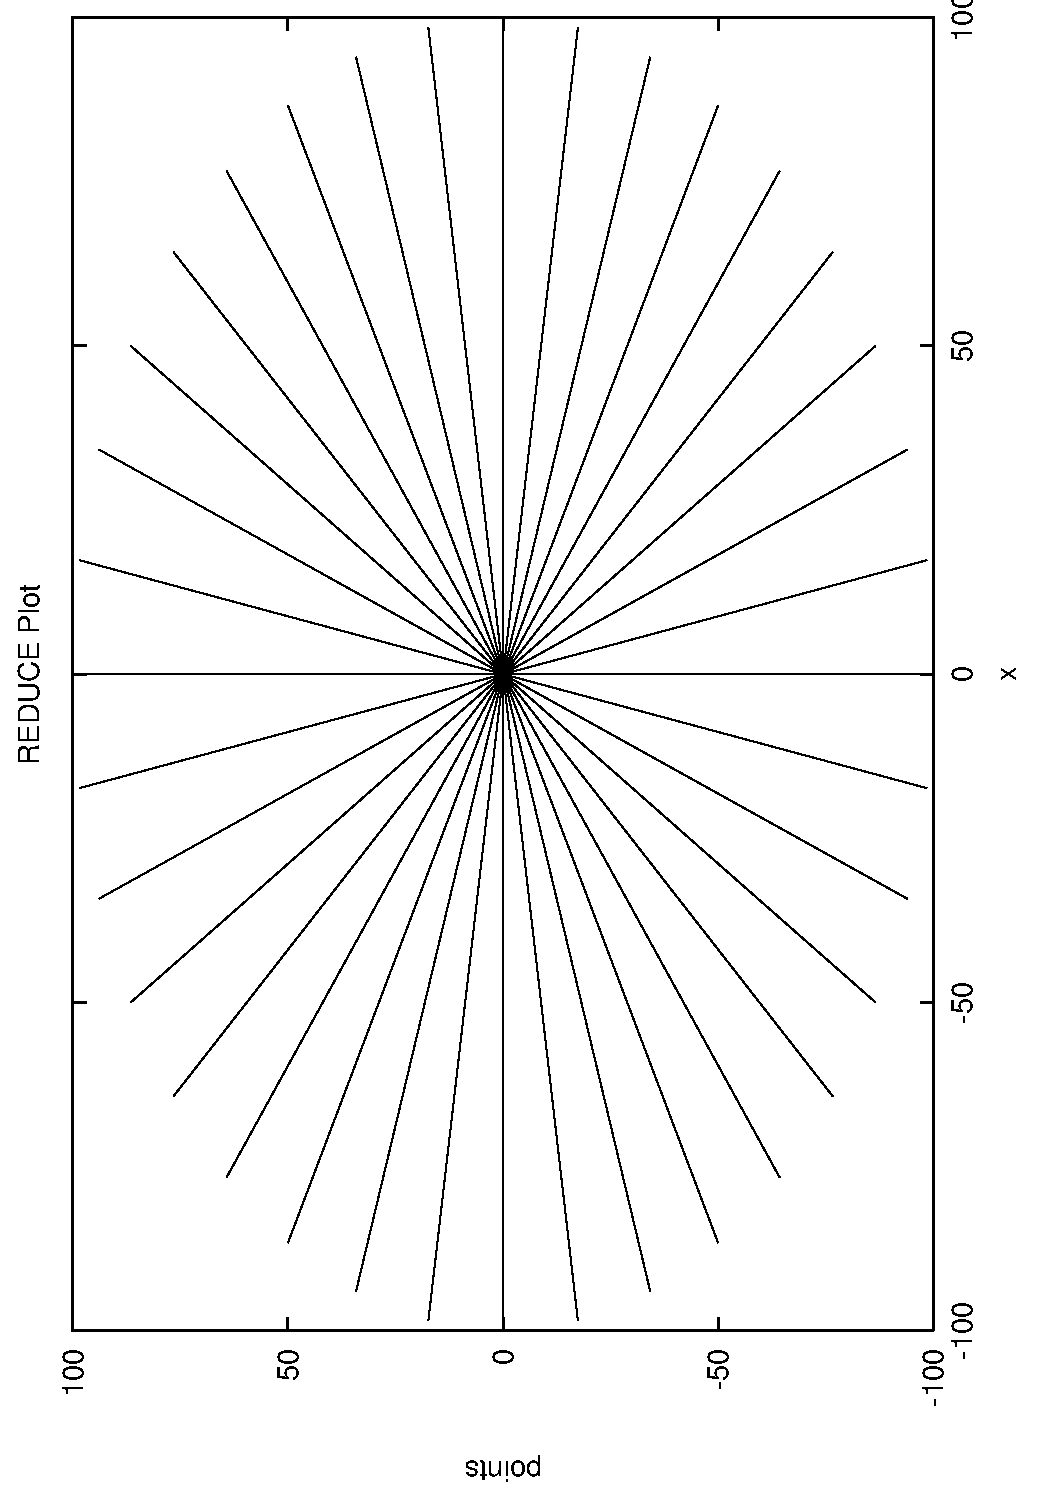
\includegraphics{eg1.pdf}}}}
\end{picture}

\begin{verbatim}
% (2) Draw 12 regular polygons with 12 sides of length 40,each polygon
%forming an angle of 360/n degrees with the previous one. 

draw {for i:=1:12 collect
          {turnleft(30), for j:=1:12 collect
                             {forward 40, turnleft(30)}} };
\end{verbatim}

\unitlength=1cm
\begin{picture}(8,8)(0,0)
\put (0,8){\rotatebox{270}{\resizebox{8cm}{8cm}{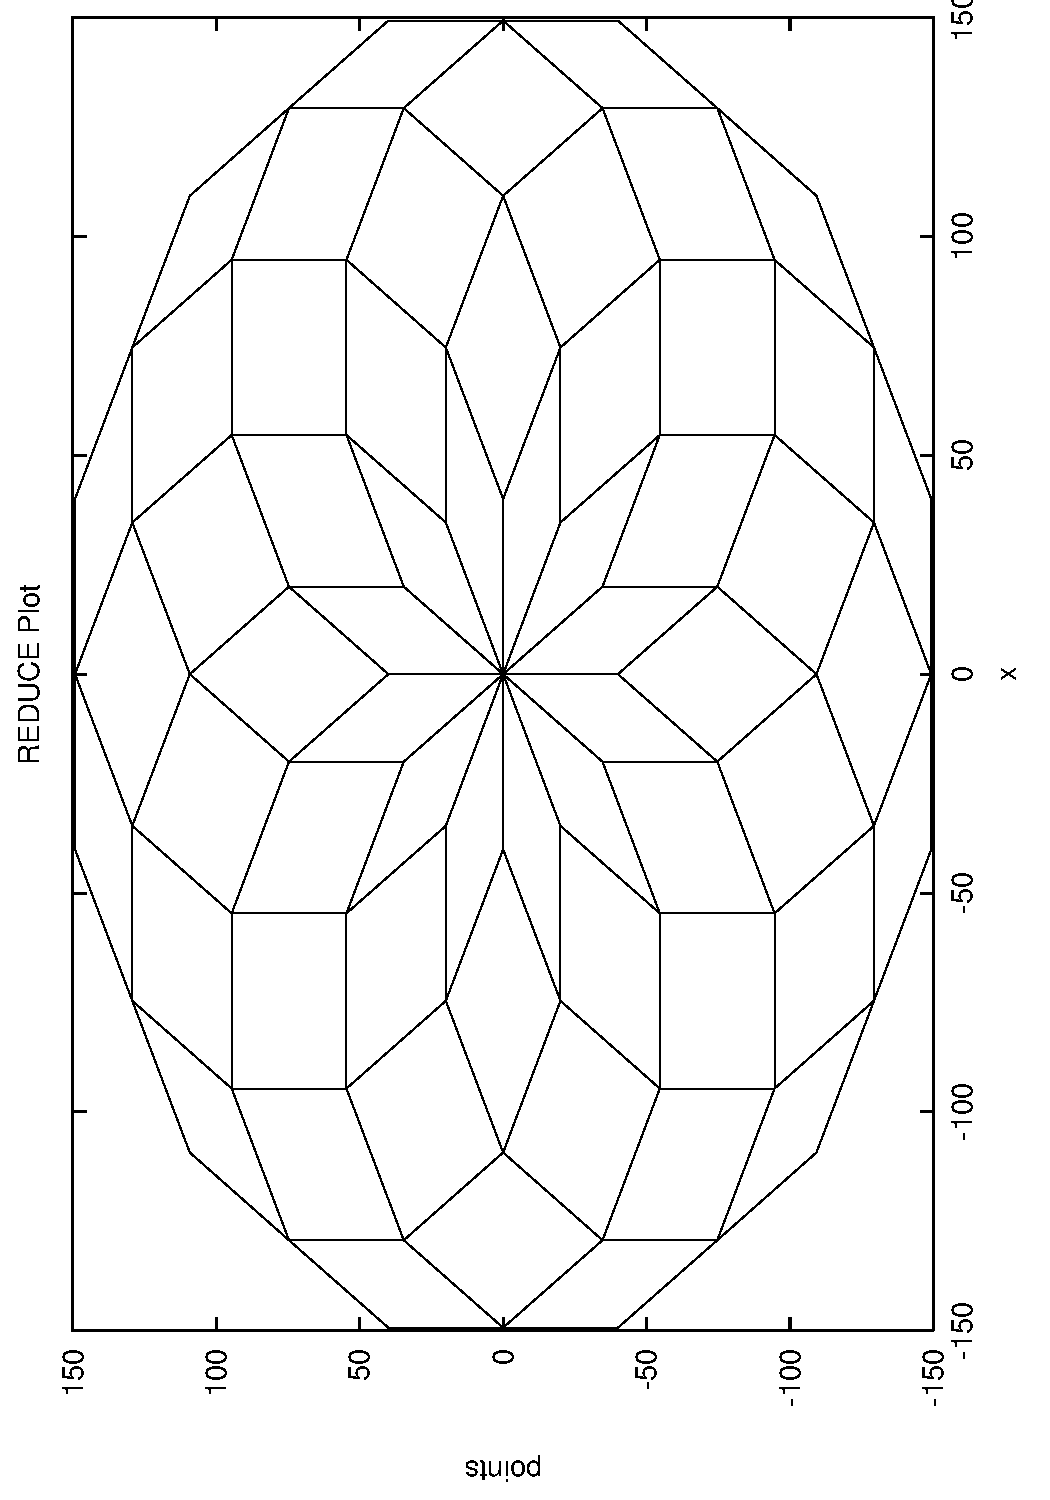
\includegraphics{eg4.pdf}}}}
\end{picture}

\begin{verbatim}
% (3) A "peak" pattern - an example of a recursive procedure.

procedure peak(r);
begin;
  return for i:=0:r collect
             {move(x_coord+5,y_coord-10), move(x_coord+10,y_coord+60),
              move(x_coord+10,y_coord-60),move(x_coord+5,y_coord+10)};
end;

draw {home(), peak(3)};
\end{verbatim}

\unitlength=1cm
\begin{picture}(8,8)(0,0)
\put (0,8){\rotatebox{270}{\resizebox{8cm}{8cm}{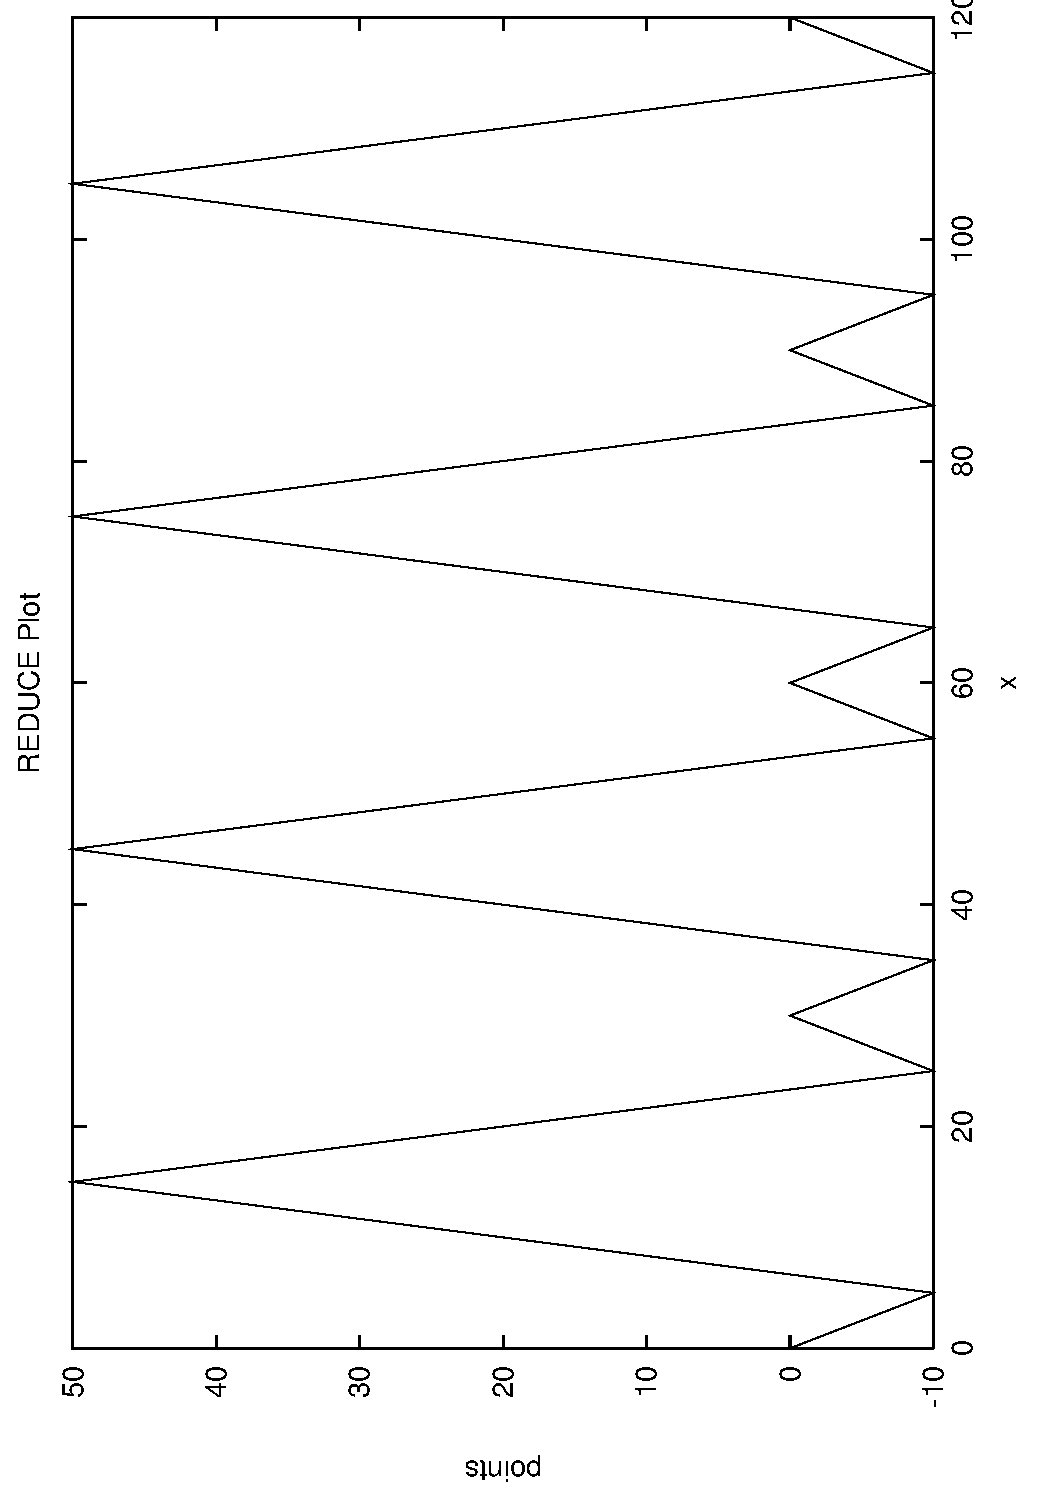
\includegraphics{eg5a.pdf}}}}
\end{picture}  

\begin{verbatim}
%This procedure can then be part of a longer chain of commands:

draw {home(), move(5,50), peak(3), move(x_coord+10,-100),
      peak(2), move(x_coord+10,0)};
\end{verbatim}

\unitlength=1cm
\begin{picture}(8,8)(0,0)
\put (0,8){\rotatebox{270}{\resizebox{8cm}{8cm}{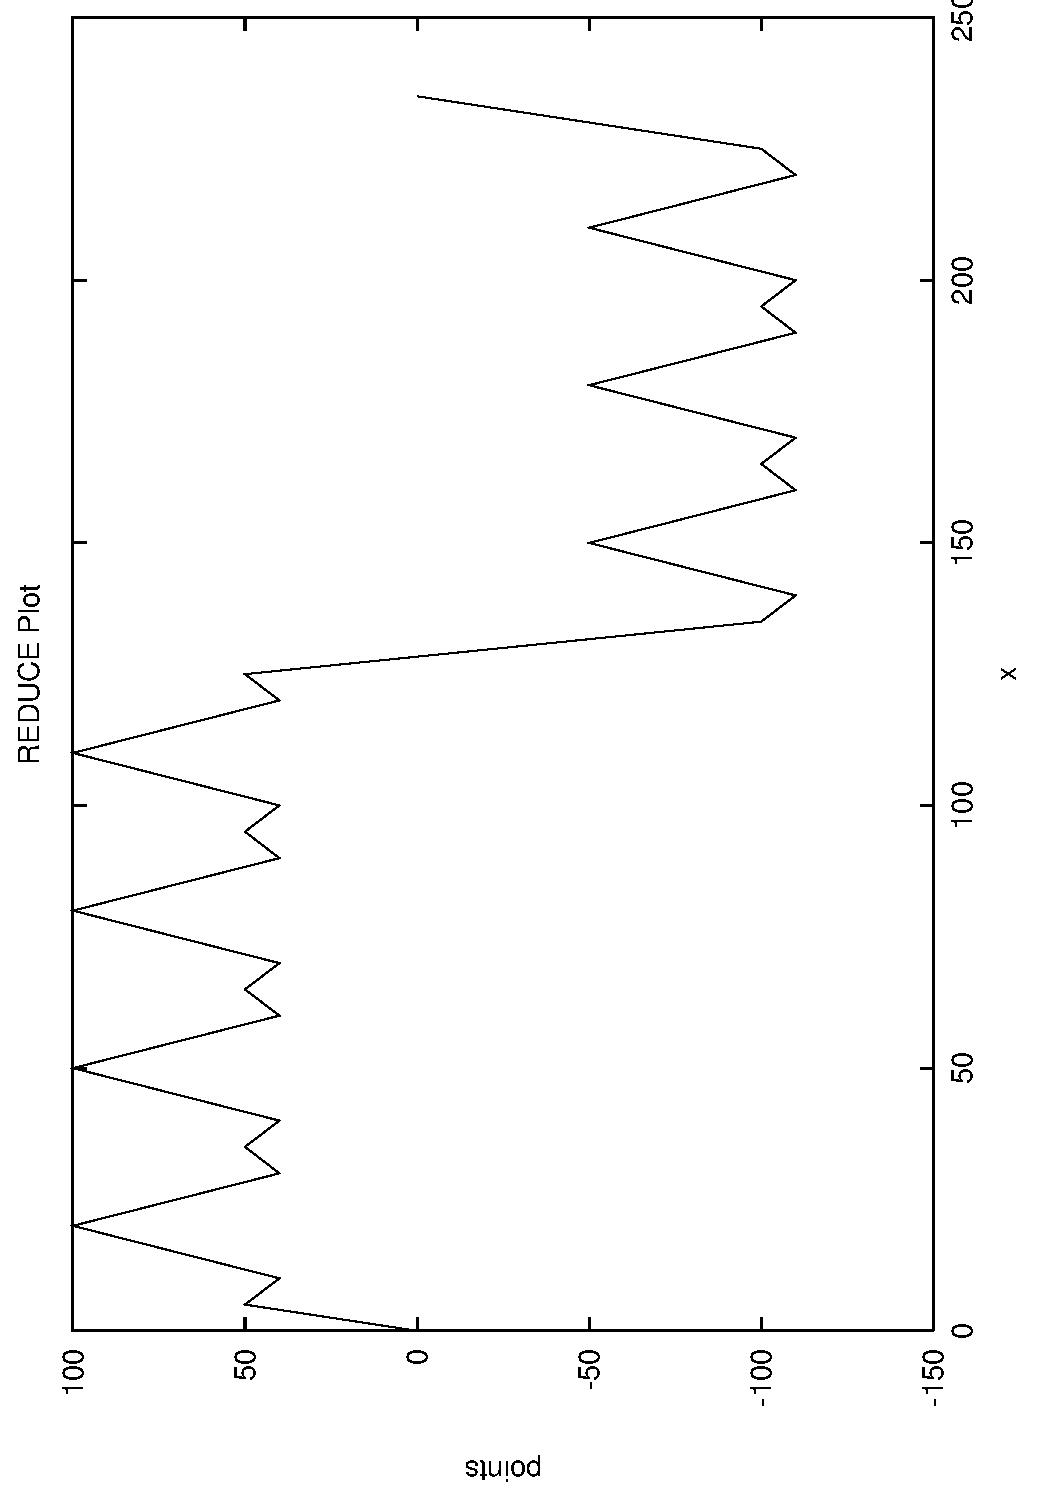
\includegraphics{eg5b.pdf}}}}
\end{picture}  

\begin{verbatim}
% (4)  Write a recursive procedure which draws "trees" such that every
%branch is half the length of the previous branch.

procedure tree(a,b);         %Here: a is the start length, b is the
                             %number of levels
begin;
  return if fixpb and b>0           %checking b is a positive integer

            then {turnleft(45), forward a, tree(a/2,b-1),
                  back a, turnright(90), forward a, tree(a/2,b-1),
                  back a, turnleft(45)}
         else {x_coord,y_coord};    %default: Turtle stays still
end;

draw {home(), tree(130,7)};
\end{verbatim}

\unitlength=1cm
\begin{picture}(8,8)(0,0)
\put(0,8){\rotatebox{270}{\resizebox{8cm}{8cm}{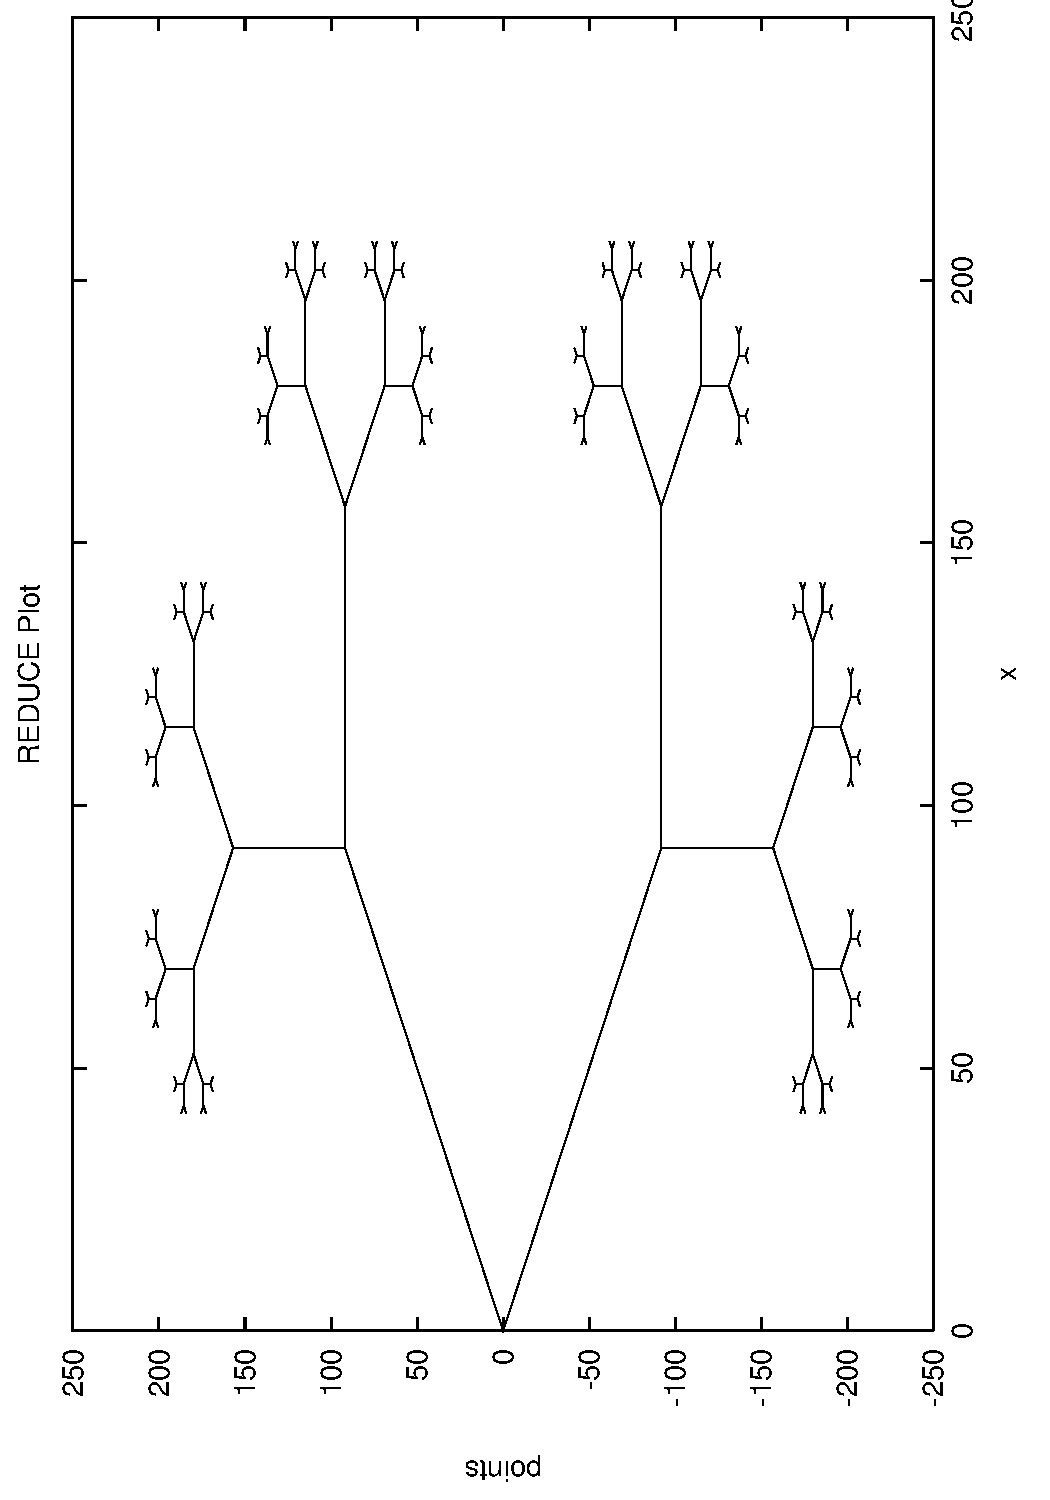
\includegraphics{eg6a.pdf}}}}
\end{picture}  

\begin{verbatim}
% (5)  A 36-point star.

draw {home(), for i:=1:36 collect
                  {turnleft(10), forward 100, turnleft(10), back 100} };
\end{verbatim}

\unitlength=1cm
\begin{picture}(8,8)(0,0)
\put(0,8){\rotatebox{270}{\resizebox{8cm}{8cm}{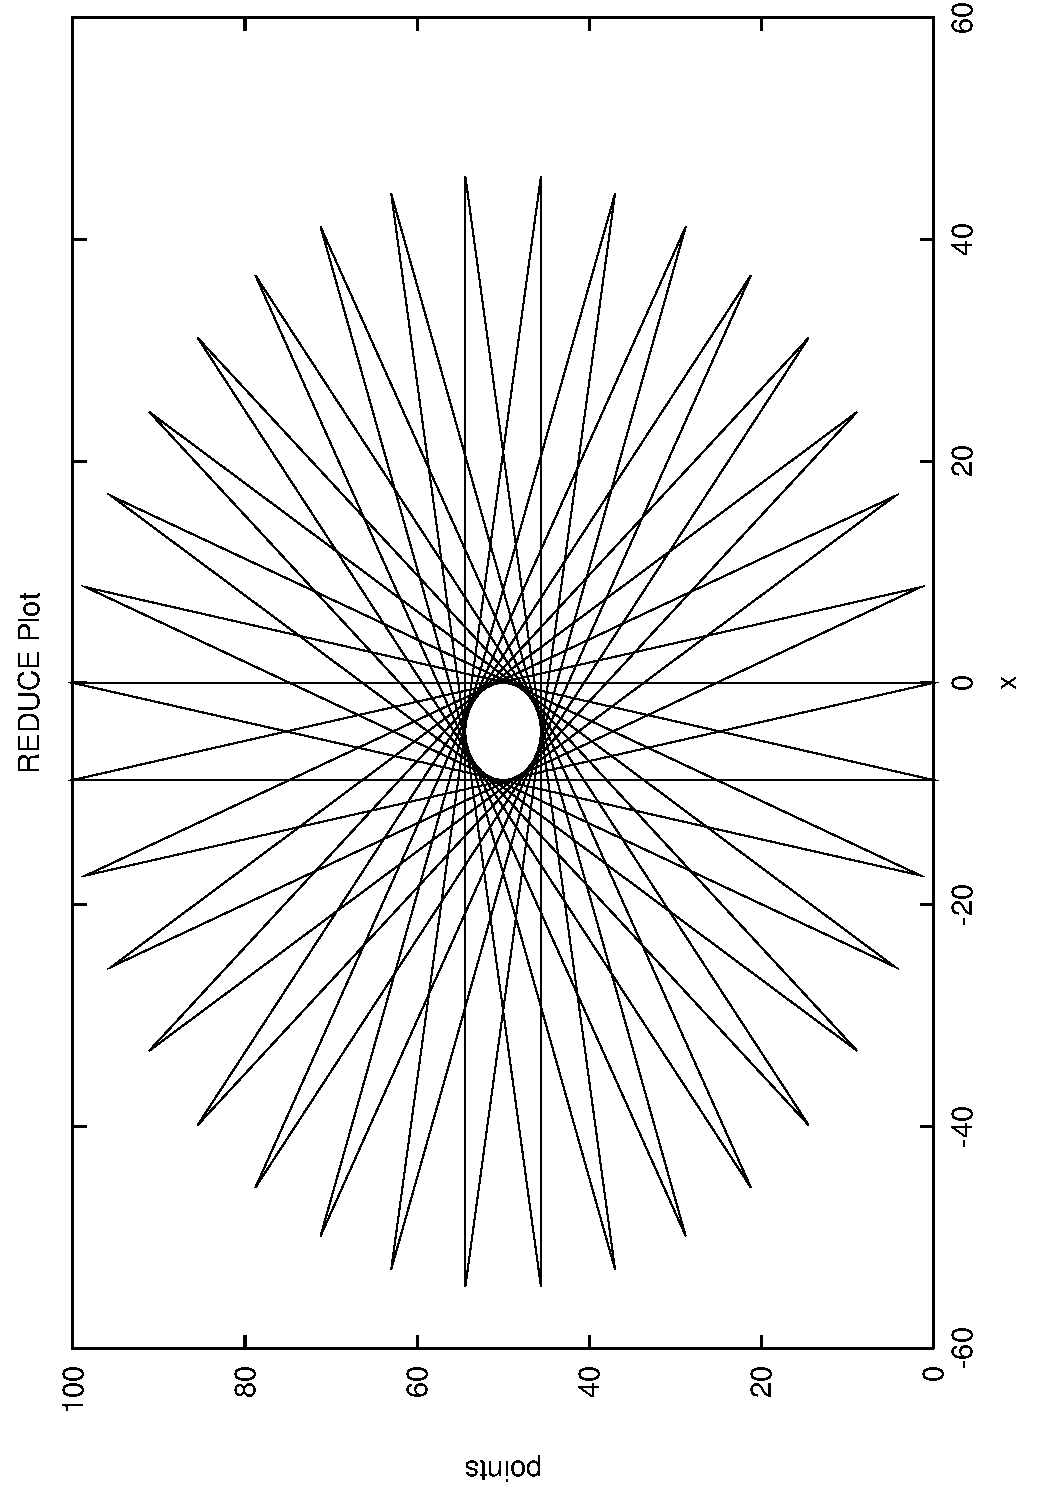
\includegraphics{eg7.pdf}}}}
\end{picture}  

\begin{verbatim}
% (6) Draw 100 equilateral triangles with the leading points
%equally spaced on a circular path.

draw {home(), for i:=1:100 collect
                  {forward 150, rightturn(60), back(150),
                   rightturn(60), forward 150, setheading(i*3.6)} };
\end{verbatim}

\unitlength=1cm
\begin{picture}(8,8)(0,0)
\put(0,8){\rotatebox{270}{\resizebox{8cm}{8cm}{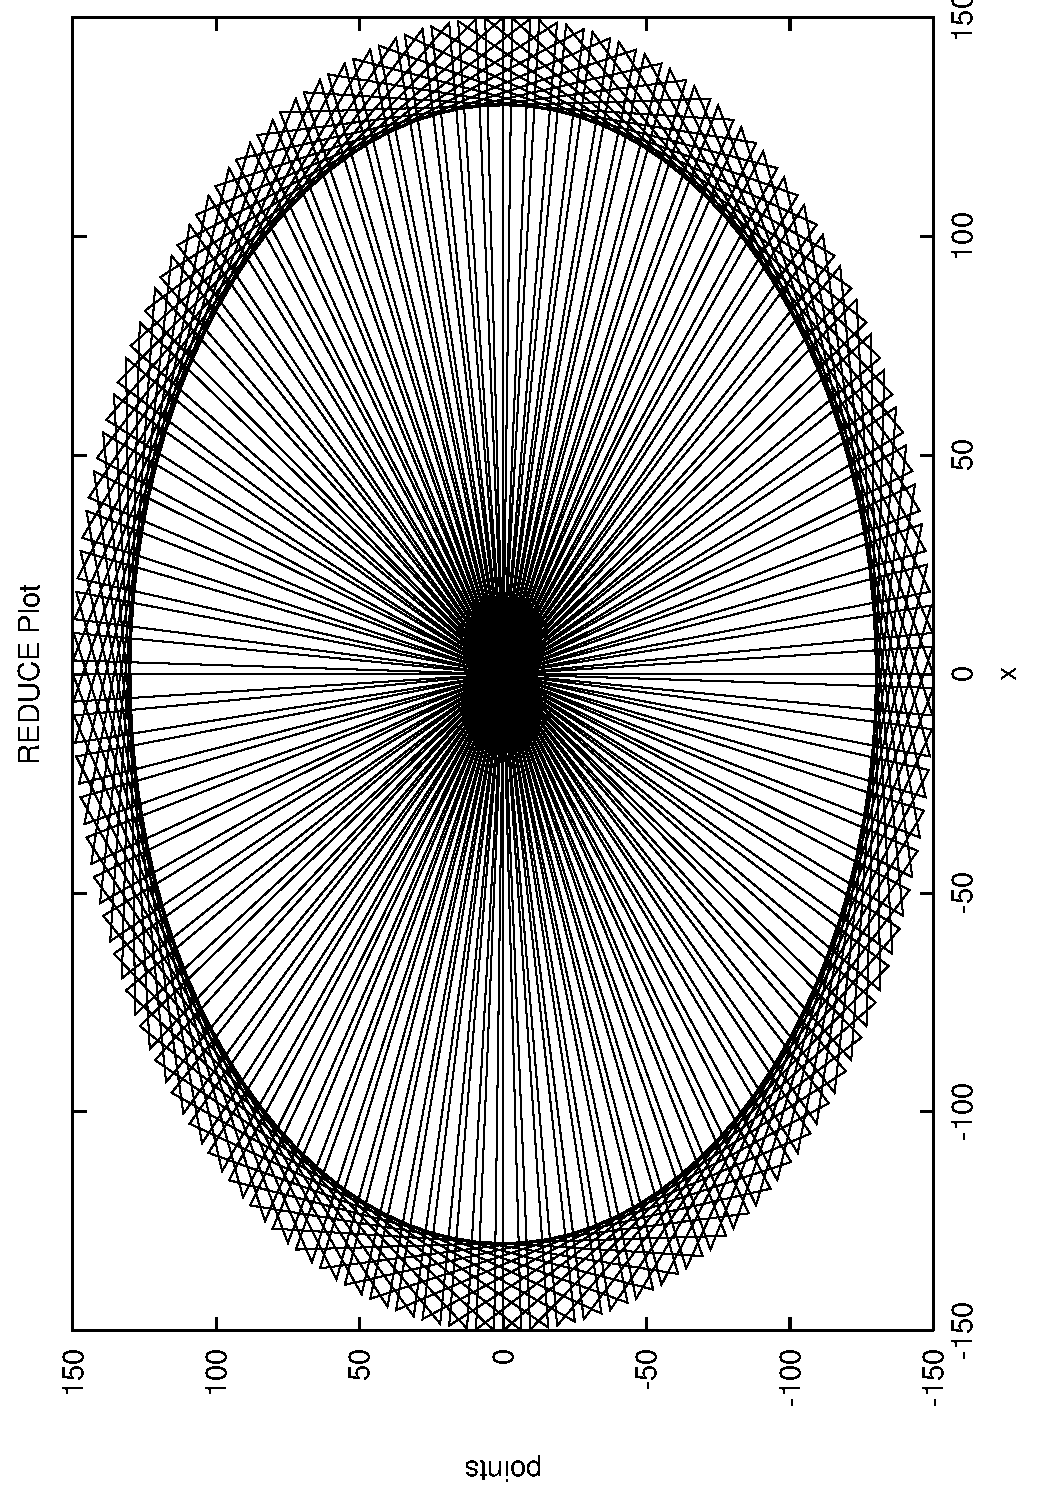
\includegraphics{eg8.pdf}}}}
\end{picture}  

\begin{verbatim}
% (7) Two or more graphs can be drawn together (this is easier
%if the graphs are named). Here we show graphs 2 and 6 on top of one
%another:

gr2:={home(), for i:=1:12 collect
                  {turnleft(30), for j:=1:12 collect
                                     {forward 40, turnleft(30)}} }$

gr6:={home(), for i:=1:100 collect
                  {forward 150, turnright(60), back(150),
                   turnright(60), forward 150, setheading(i*3.6)} }$

draw {gr2, gr6};
\end{verbatim}

\unitlength=1cm
\begin{picture}(8,8)(0,0)
\put(0,8){\rotatebox{270}{\resizebox{8cm}{8cm}{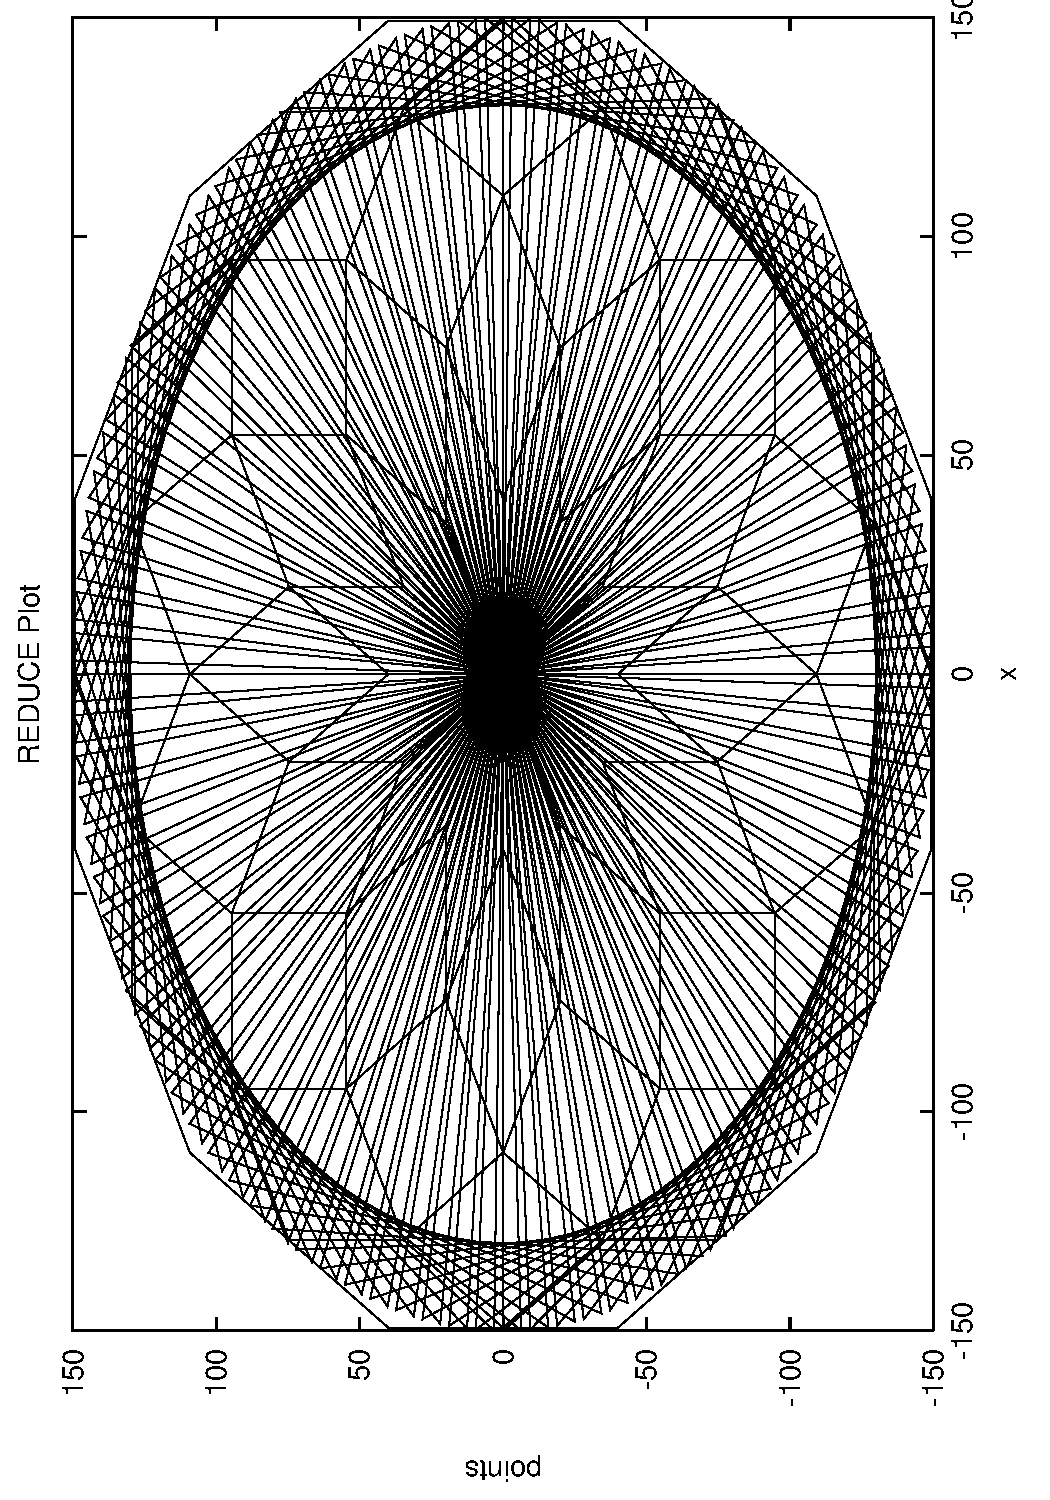
\includegraphics{eg9.pdf}}}}
\end{picture}  

\begin{verbatim}
% (8) Example 7 could have been tackled another way, which makes use of 
%the fdraw command.
%By inputting gr2 and gr6 as procedures into reduce, they can then be 
%used at any time in the same reduce session in a call to draw and even
%fdraw.

%First save the procedures in a file, say fxp (fdraw example procedures):

procedure gr2;
begin;
  return {home, for i:=1:12 collect
                    {leftturn(30), for j:=1:12 collect
                                       {forward 40, leftturn(30)}} };
end;

procedure gr6;
begin;
  return {home(), for i:=1:100 collect
                  {forward 150, rightturn(60), back(150),
                   rightturn(60), forward 150, setheading(i*3.6)} };
end;

%Then create another file where the functions may be called to fdraw,
%e.g. fx:

gr2
gr6

%Now in reduce, after loading the turtle package just type the following:

in "fxp";
fdraw '"fx";

%..and the graphs will appear.

%This method is useful if the user wants to define many of their own
%functions, and, using fdraw, subtle changes can be made quickly without 
%having to type out the whole string of commands to plot each time. It 
%is particularly useful if there are several pictures to plot at once and 
%it is an easy way to build pictures so that the difference an extra 
%command makes to the overall picture can be clearly seen.
%(In the above example, the file called to fdraw was only 2 lines long,
%so this method did not have any advantage over the normal draw command. 
%However, when the list of commands is longer it is clearly advantageous 
%to use fdraw)


\end{verbatim}


\section{References}

\begin{enumerate}
 \item {\bf An Implementation of Turtle Graphics for Teaching Purposes}\\
         Zoran I. Putnik \& Zoram d.Budimac

 \item {\bf Mapletech -} Maple in Mathematics and the Sciences,\\ 
        Special Issue 1994\\
       {\bf An Implementation of ``Turtle Graphics'' in Maple V}\\
         Eugenio Roanes Lozano \&  Eugenio Roanes Macias

\end{enumerate}

\end{document}


